\section{Menús}

\subsection{Menú principal}
Esta es el menú que ve el jugador cuando abre el juego. Desde él se puede modificar el nombre (que se mostrará en partida), elegir el personaje a jugar en la siguiente partida, buscar partida, ver información sobre los personajes y cambiar las opciones de sonido.

\vspace{\baselineskip}

\begin{figure}[H]
	\centering
	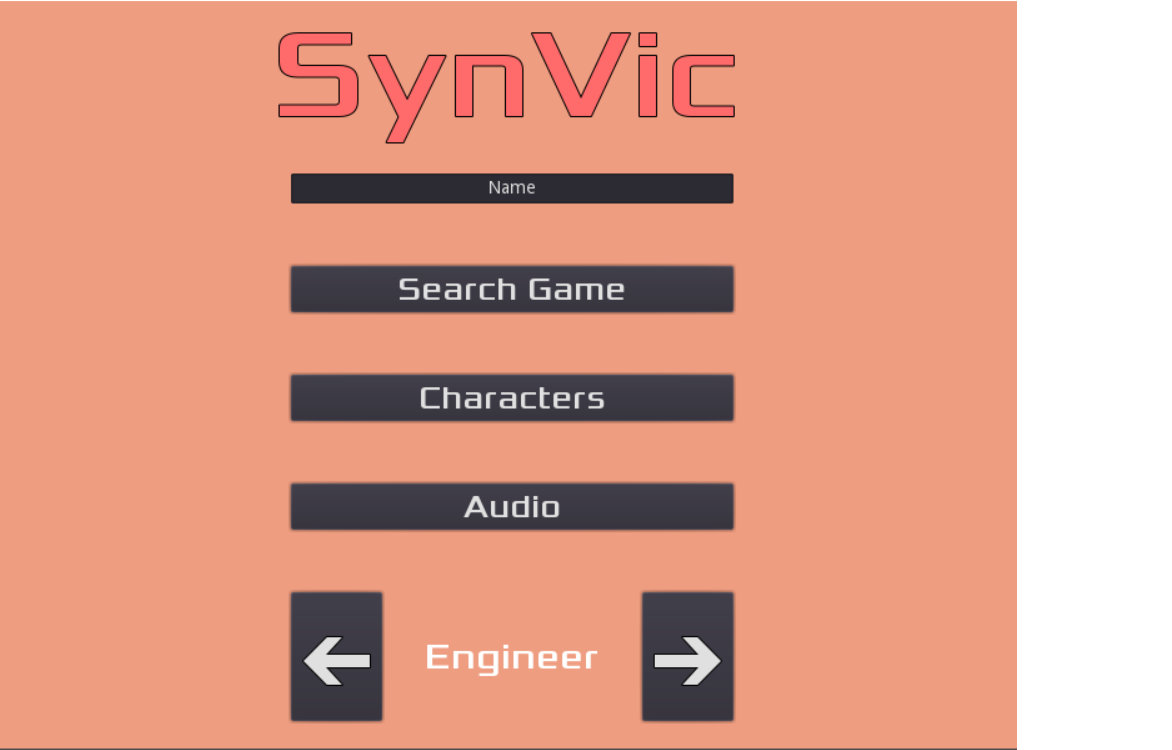
\includegraphics[width=0.7\linewidth]{figures/MainMenu}
	% \caption{Menú principal del juego.}
	\label{fig:MainMenu}
\end{figure}

\vspace{\baselineskip}
\vspace{\baselineskip}

\subsection{Menú de Sonido}
Permite configurar de forma separada el volumen maestro (que afecta a todo el sonido del juego), el volumen de la música y el volumen de los efectos de sonido. Además, se puede directamente silenciar cada uno de estos volúmenes por separado.

\vspace{\baselineskip}

\begin{figure}[H]
	\centering
	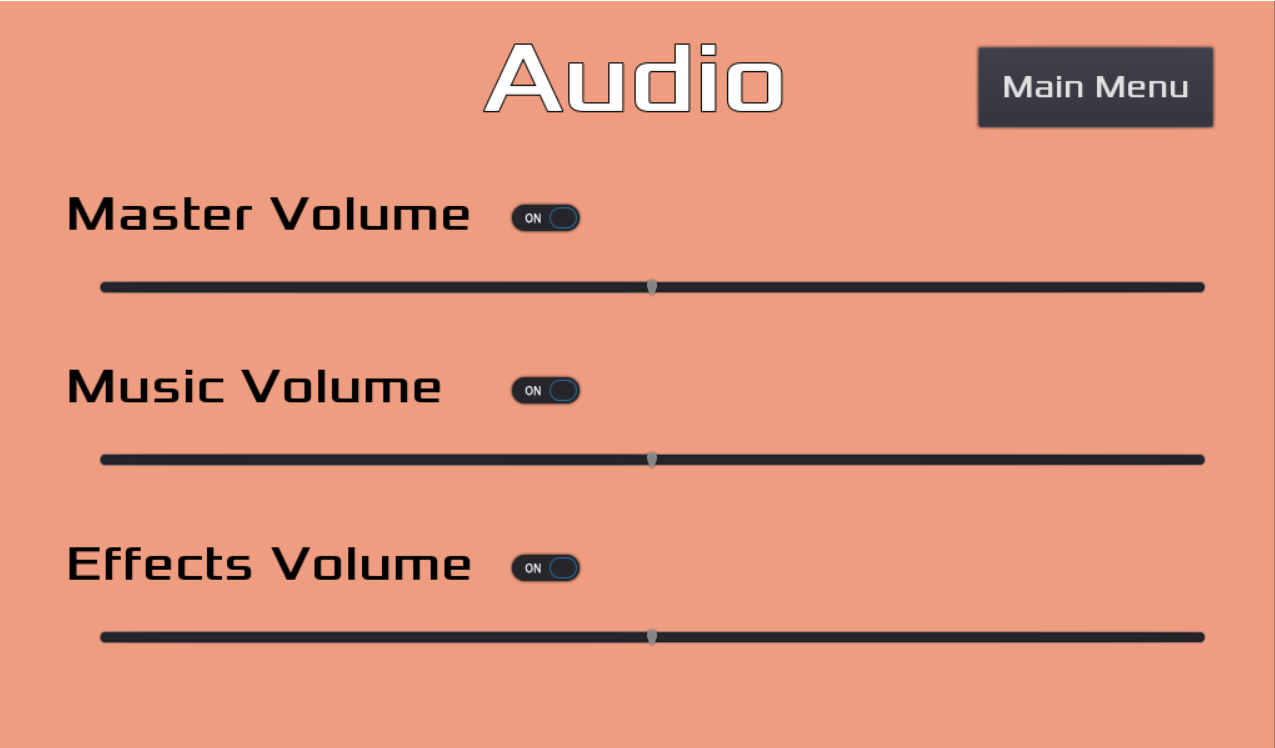
\includegraphics[width=0.7\linewidth]{figures/AudioMenu}
	% \caption{Menú de configuración de sonido.}
	\label{fig:AudioMenu2}
\end{figure}

\newpage

\subsection{Menú de Personajes}
En este menú se puede acceder a la información sobre cualquier personaje, incluyendo el funcionamiento de sus habilidades.

\vspace{\baselineskip}

\begin{figure}[H]
	\centering
	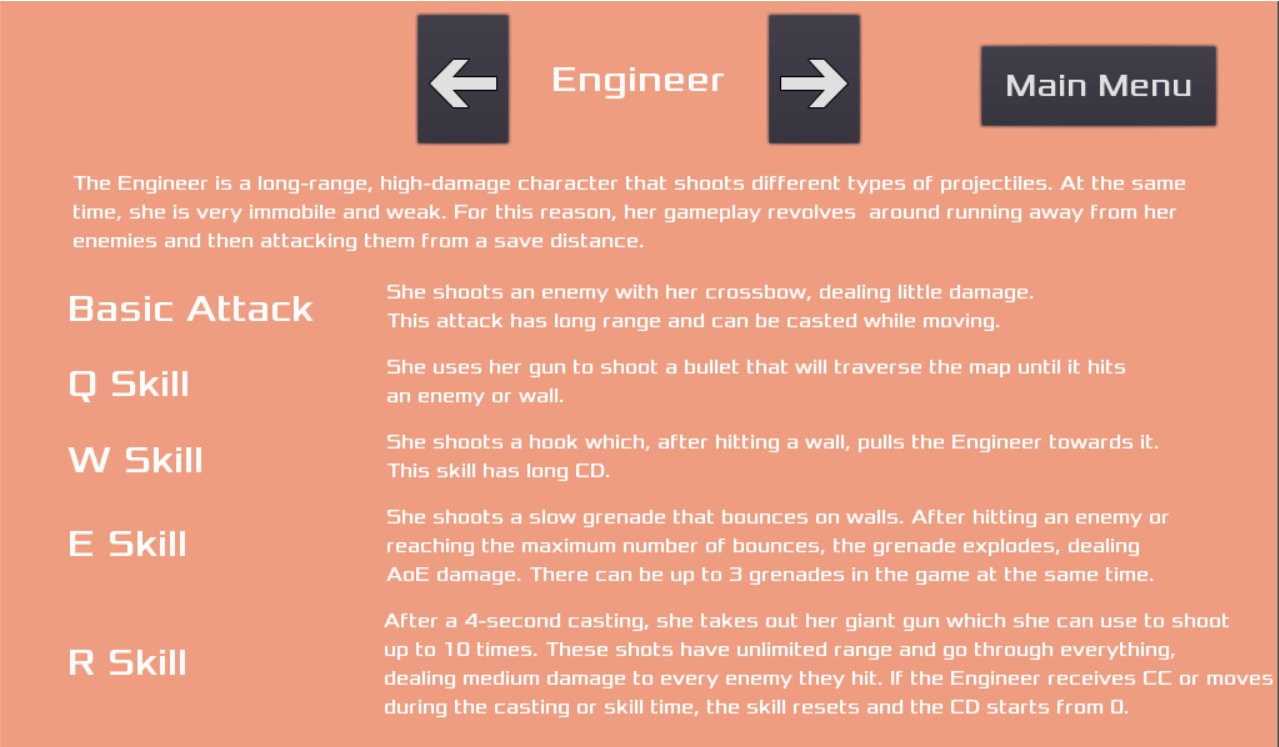
\includegraphics[width=0.7\linewidth]{figures/CharacterMenu}
	% \caption{Menú de personajes.}
	\label{fig:CharacterMenu}
\end{figure}

\vspace{\baselineskip}
\vspace{\baselineskip}

\subsection{Lobby}
Tras encontrar una partida, se accede al Lobby junto a otros tres jugadores. En el Lobby se muestra el tipo de partida (mapa) a jugar y se votan para elegir equipos en función de los distintos personajes. Cada jugador puede votar (\emph{botón flecha arriba}) a otro jugador para que sea su compañero de equipo y a otro (\emph{botón X}) para que \textbf{no} sea su compañero de equipo. En función de esta votación, se forman los equipos.

\vspace{\baselineskip}

\begin{figure}[H]
	\centering
	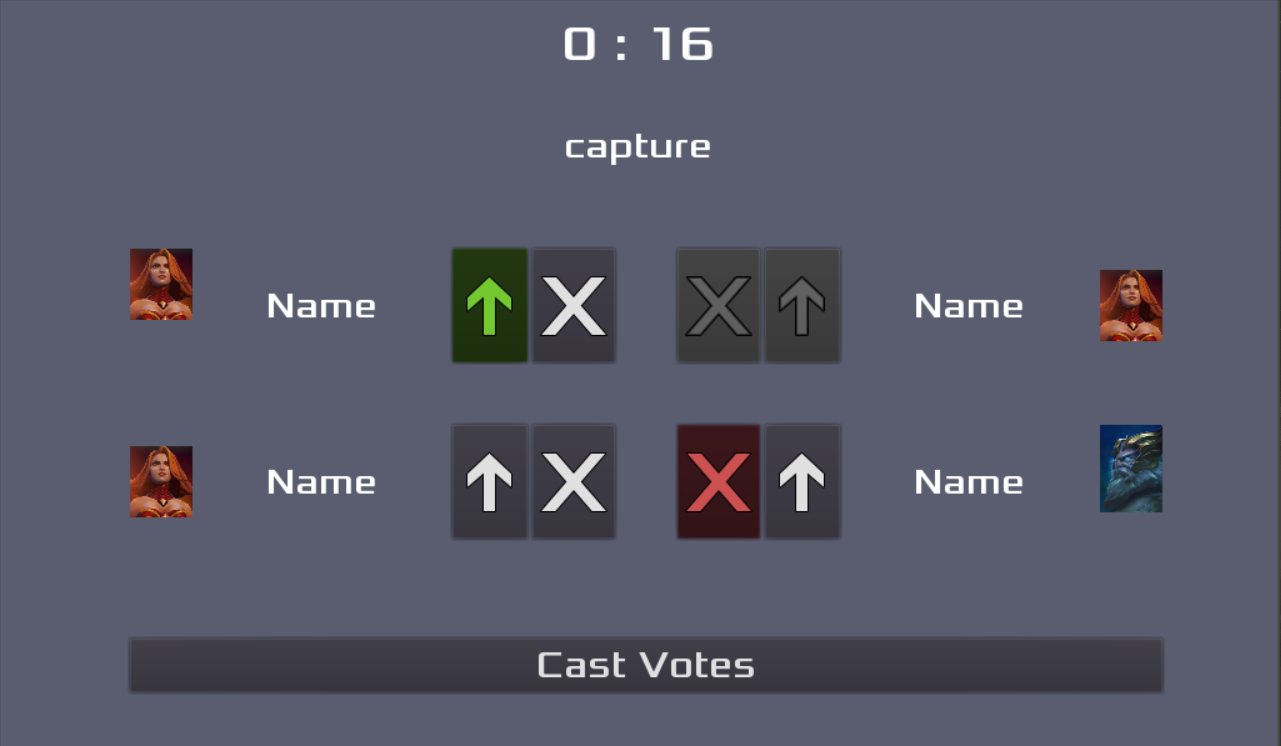
\includegraphics[width=0.7\linewidth]{figures/Lobby}
	% \caption{Lobby.}
	\label{fig:Lobby}
\end{figure}